\DTLloaddb[noheader, keys={key,value}]{data_col}{data_col.txt}
\renewcommand{\var}[1]{\DTLfetch{data_col}{key}{#1}{value}}
\section{Dise\~no de columnas}
    Se dise\~nará la columna presentada a continuaci\'on
    Geometr\'ia de la columna:
    \begin{itemize}
        \item Ancho: b = \var{b} cm
        \item Peralte: h = \var{h} cm  
    \end{itemize}

    Datos de los materiales:

    Datos del refuezo:
    \begin{itemize}
        \item Recubrimiento: $r_e = \var{r_e} cm$
        \item Di\'ametro del acero longitudinal: $d_b = \var{d_b}$
        \item Di\'ametro de estribos:$ d_e = \var{d_e}$       
    \end{itemize}

    \subsection{Dise\~no por flexi\'on y carga axial}
    La resistencia m\'axima de dise\~no a compresi\'on ser\'a:
    \[ \phi P_n = 0.80 \cdot \phi_{com} \cdot [0.85 \cdot f'_c \cdot (A_g-A_{st})+f_y \cdot A_{st}] \]
    \[ \phi P_n = 0.85 \cdot \var{phi_c} \cdot [0.85 \cdot \var{f_c} \cdot (\var{A_g}-\var{A_st})+\var{f_y} \cdot \var{A_st}] = \var{P_n} \] \\


    Cargas sometidas a la columna:\\
    \begin{tabular}{lrrr}
\toprule
Combinacion &            P &         M2 &         M3 \\
\midrule
       1.4D &  -127502.532 & -13109.103 & -37897.992 \\
       1.4D &  -110630.313 &  10006.200 &  56115.162 \\
       1.4D &  -277824.105 & -10789.038 & -43266.024 \\
       1.4D &  -260951.886 &   4777.470 &  28345.014 \\
       1.4D &  -429920.307 &  -8866.278 & -45508.590 \\
       1.4D &  -413048.088 &   4117.257 &  27897.678 \\
       1.4D &  -582035.148 &  -7961.796 & -44780.688 \\
       1.4D &  -565162.929 &   3724.857 &  26709.687 \\
       1.4D &  -733437.783 &  -6946.461 & -56010.195 \\
       1.4D &  -716565.564 &   2536.866 &  23631.309 \\
       1.4D &  -909355.608 &  -3005.784 & -10745.874 \\
       1.4D &  -870852.339 &   1785.420 &  33757.191 \\
  1.2D+1.6L &  -128712.105 & -11286.405 & -59613.408 \\
  1.2D+1.6L &  -114250.203 &  11640.546 &  54711.351 \\
  1.2D+1.6L &  -318571.902 & -11462.004 & -55777.698 \\
  1.2D+1.6L &  -304110.000 &   2830.185 &  43861.491 \\
  1.2D+1.6L &  -489401.280 & -10916.568 & -57976.119 \\
  1.2D+1.6L &  -474939.378 &   5675.085 &  34984.422 \\
  1.2D+1.6L &  -660567.141 & -10077.813 & -63117.540 \\
  1.2D+1.6L &  -646105.239 &   4608.738 &  32925.303 \\
  1.2D+1.6L &  -841475.313 &  -8616.123 & -74099.835 \\
  1.2D+1.6L &  -827013.411 &   3410.937 &  32984.163 \\
  1.2D+1.6L & -1041190.236 &  -3855.330 & -13515.237 \\
  1.2D+1.6L & -1008187.434 &   2293.578 &  44552.115 \\
\bottomrule
\end{tabular}


    Diagrama de Interaci\'on en el eje d\'ebil\\
    \begin{figure}[h!]
        \centering
        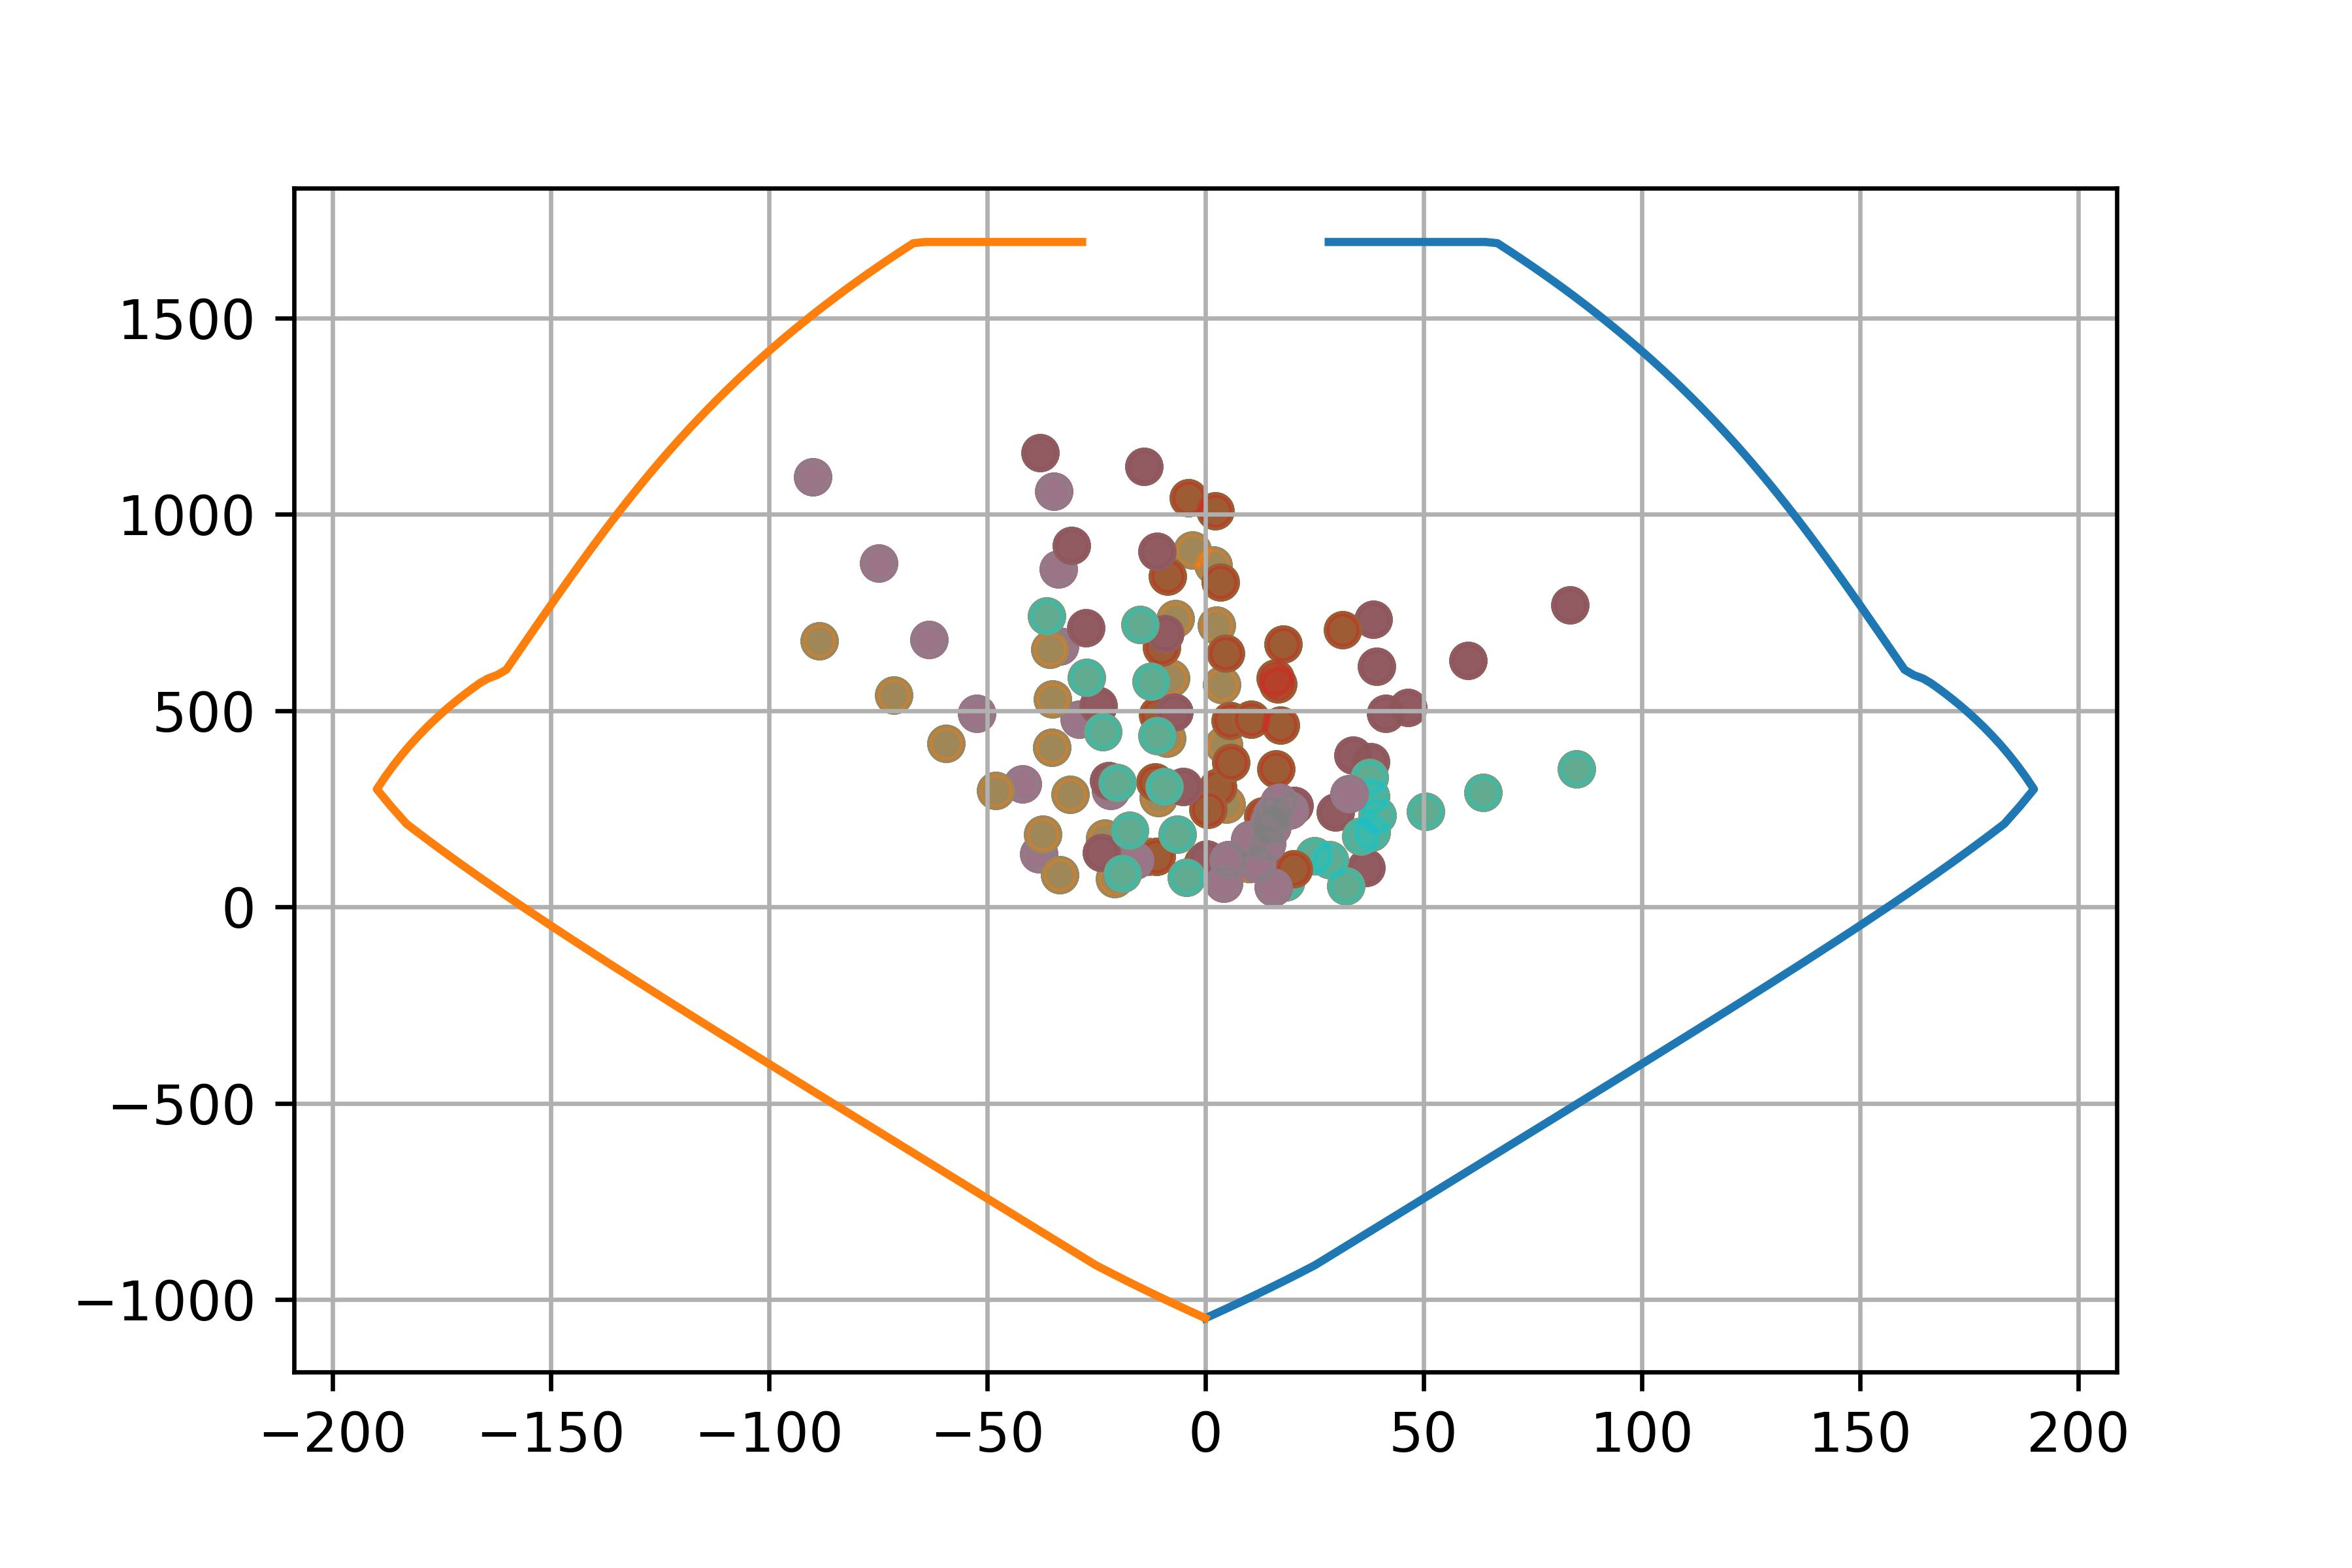
\includegraphics[scale=0.85]{diag_x.jpg}
    \end{figure}

    Diagrama de Interaci\'on en el eje fuerte\\
    \begin{figure}[h!]
        \centering
        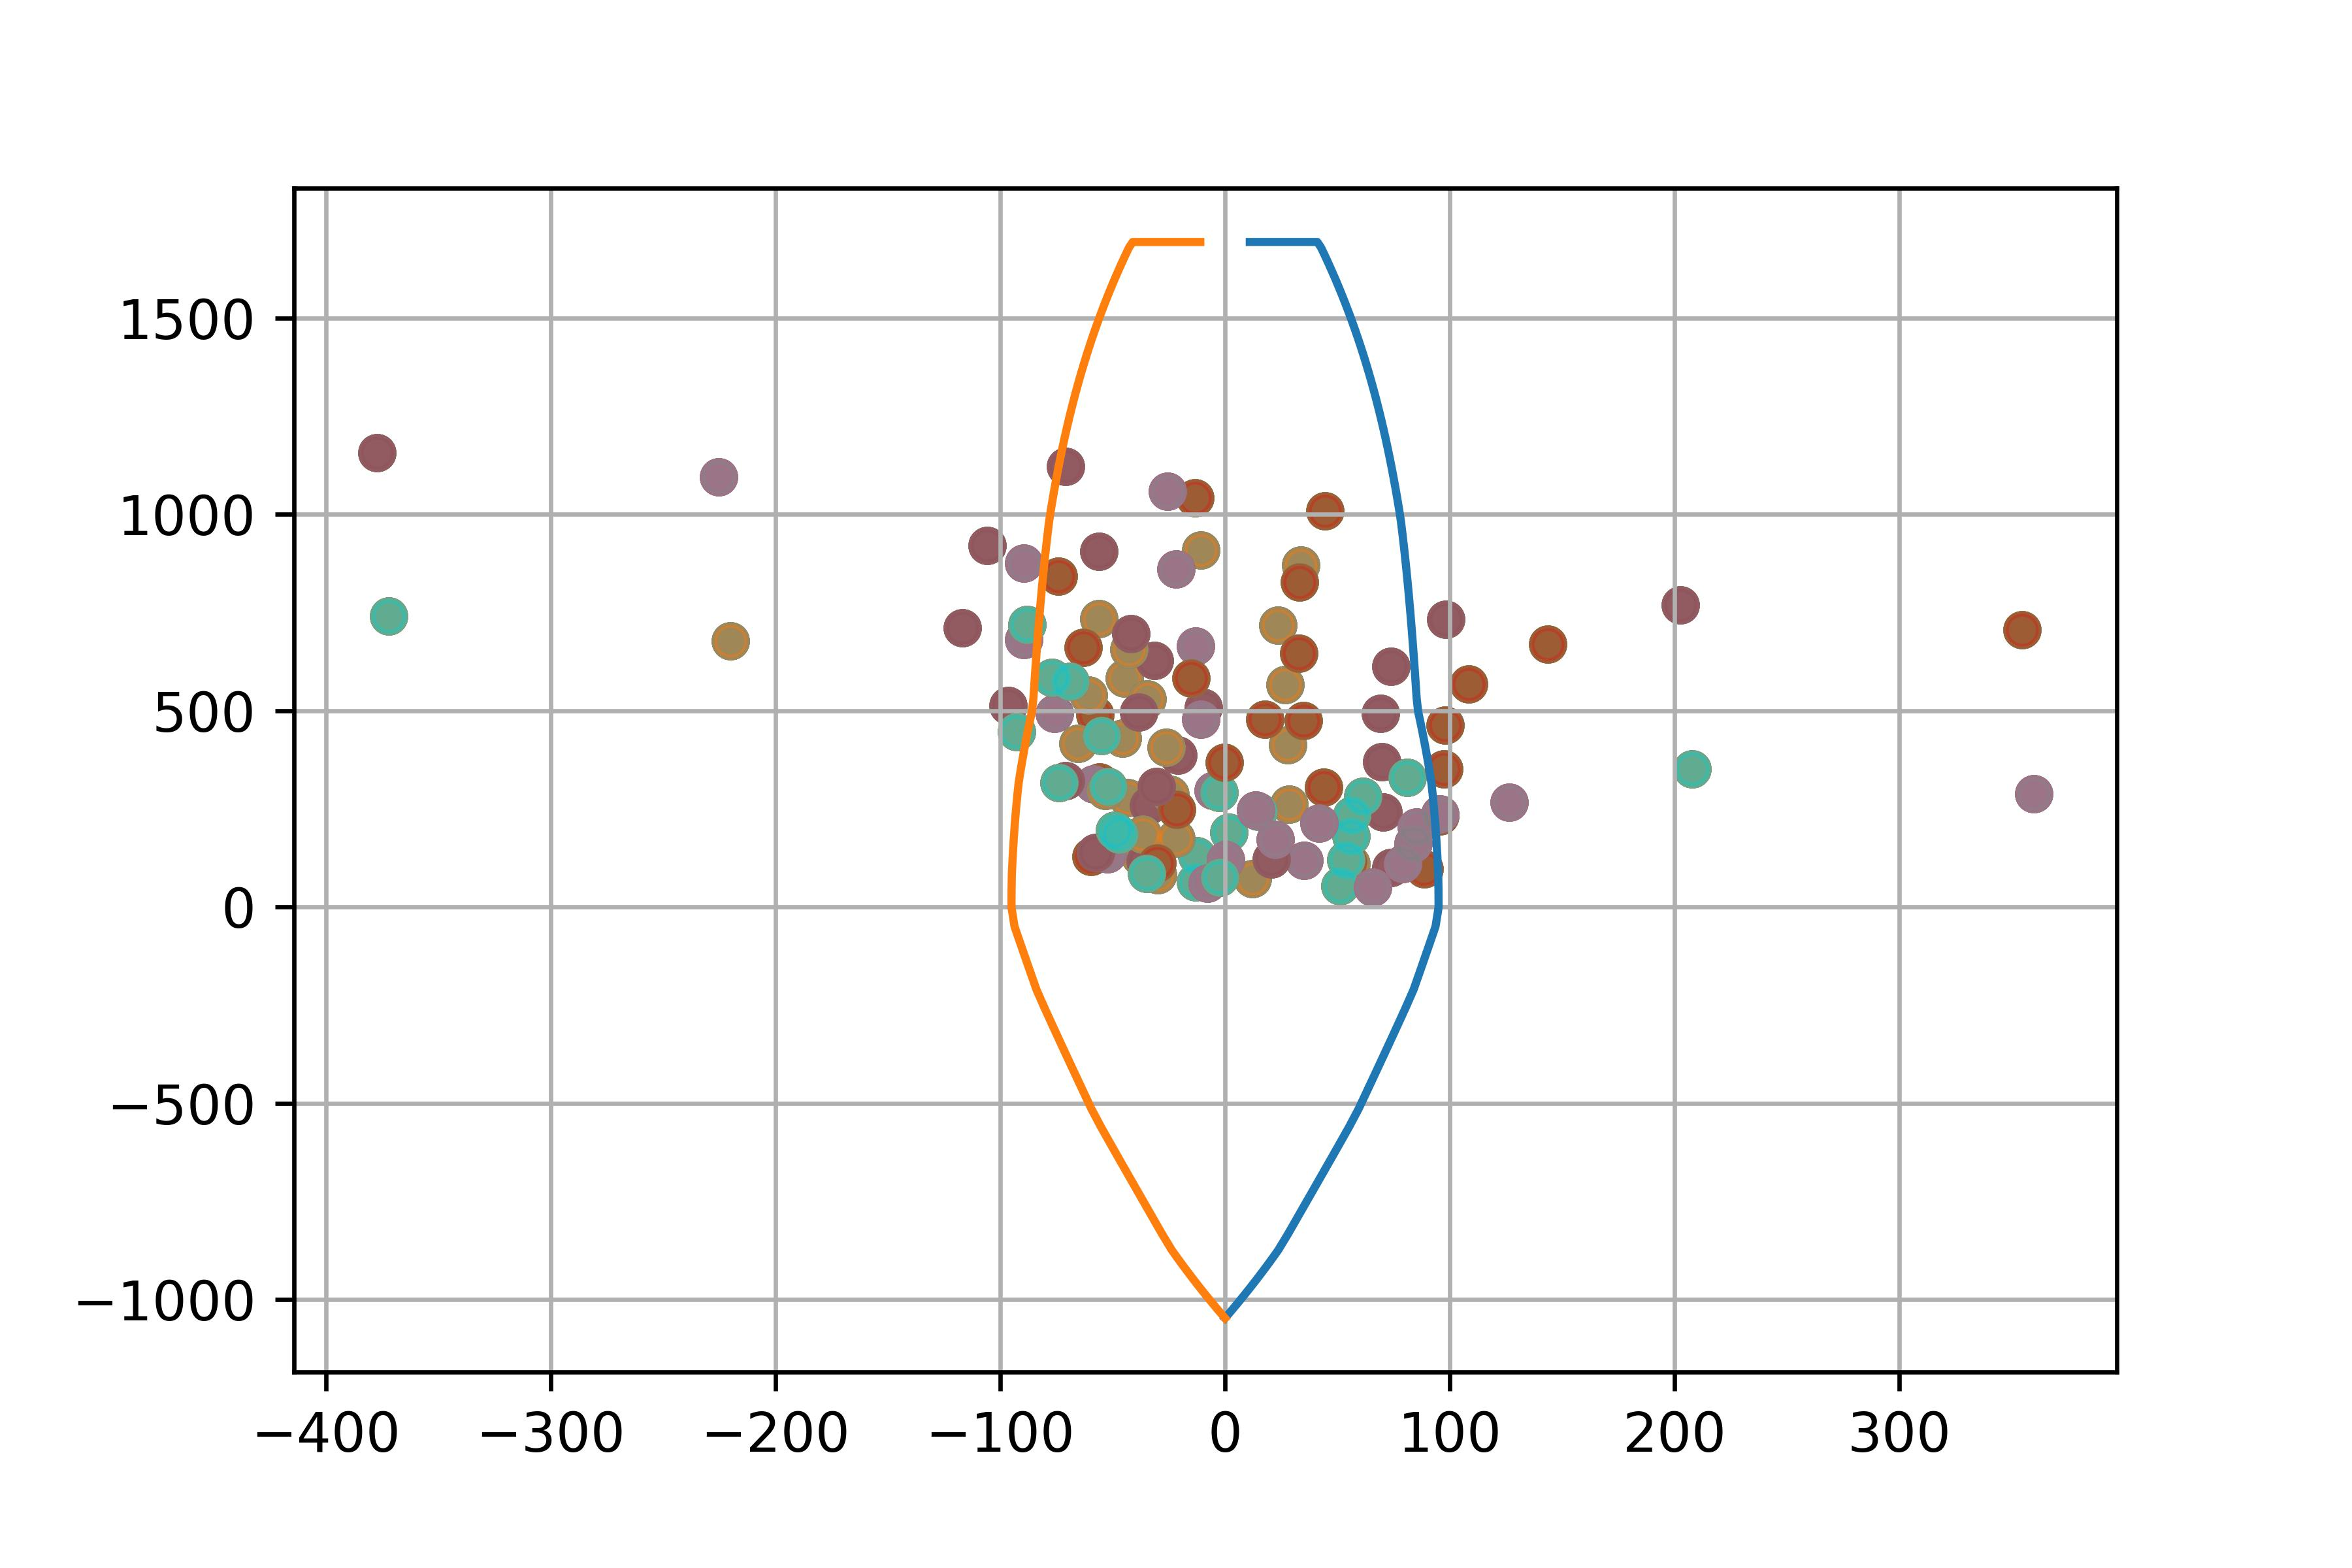
\includegraphics[scale=0.85]{diag_y.jpg}
    \end{figure}